\chapter{Physical Experimental Setup and Printable Layout Artifacts}
\label{ch:appendix_physical_setup}

\section{Overview of the Physical Setup}
\label{sec:appendix_setup_overview}
This appendix shows the physical experimental setup and printable layout files used in this research. The complete system works with a single normal RGB webcam and a sheet of plain printed paper on a flat table. No special hardware like depth cameras or sensor gloves are needed.

Figure~\ref{fig:appendix_physical_setup} shows the physical desk arrangement. A low-cost USB webcam is mounted on an adjustable desk arm above the workspace. In physical experiments, the camera elevation height $h$ varies between $14\text{ cm}$ and $28\text{ cm}$ vertically above the desk surface, while the horizontal distance $d$ from the camera mount base to the printed paper layout ranges between $14\text{ cm}$ and $28\text{ cm}$.

The camera downward viewing angle does not need manual measurement because it is calculated directly from these physical dimensions using right-angle trigonometry:
\begin{equation}
\theta = \arctan\left(\frac{h}{d}\right)
\label{eq:appendix_camera_tilt_trig}
\end{equation}
Evaluating this trigonometric relation across the operating boundary values yields:
\begin{itemize}
    \item \textbf{Minimum downward angle (lowest height and furthest distance):} For $h = 14\text{ cm}$ and $d = 28\text{ cm}$:
    \begin{equation}
    \theta_{\min} = \arctan\left(\frac{14}{28}\right) = \arctan(0.5000) \approx 26.6^\circ
    \end{equation}
    \item \textbf{Maximum downward angle (highest height and closest distance):} For $h = 28\text{ cm}$ and $d = 14\text{ cm}$:
    \begin{equation}
    \theta_{\max} = \arctan\left(\frac{28}{14}\right) = \arctan(2.0000) \approx 63.4^\circ
    \end{equation}
\end{itemize}
This gives a downward pitch angle between $26.6^\circ$ and $63.4^\circ$ relative to the horizontal desk plane (corresponding to a perspective tilt of $26.6^\circ$ to $63.4^\circ$ relative to the surface normal). The direct optical line-of-sight Euclidean distance $R = \sqrt{h^2 + d^2}$ spans from $\sqrt{14^2 + 14^2} \approx 19.8\text{ cm} \approx 20\text{ cm}$ (closest) to $\sqrt{28^2 + 28^2} \approx 39.6\text{ cm} \approx 40\text{ cm}$ (maximum). The printed paper keyboard layout is placed flat on the table, and the four AprilTag fiducial markers on the borders remain clearly visible to the camera during single-handed interaction.

\begin{figure}[htbp]
\centering
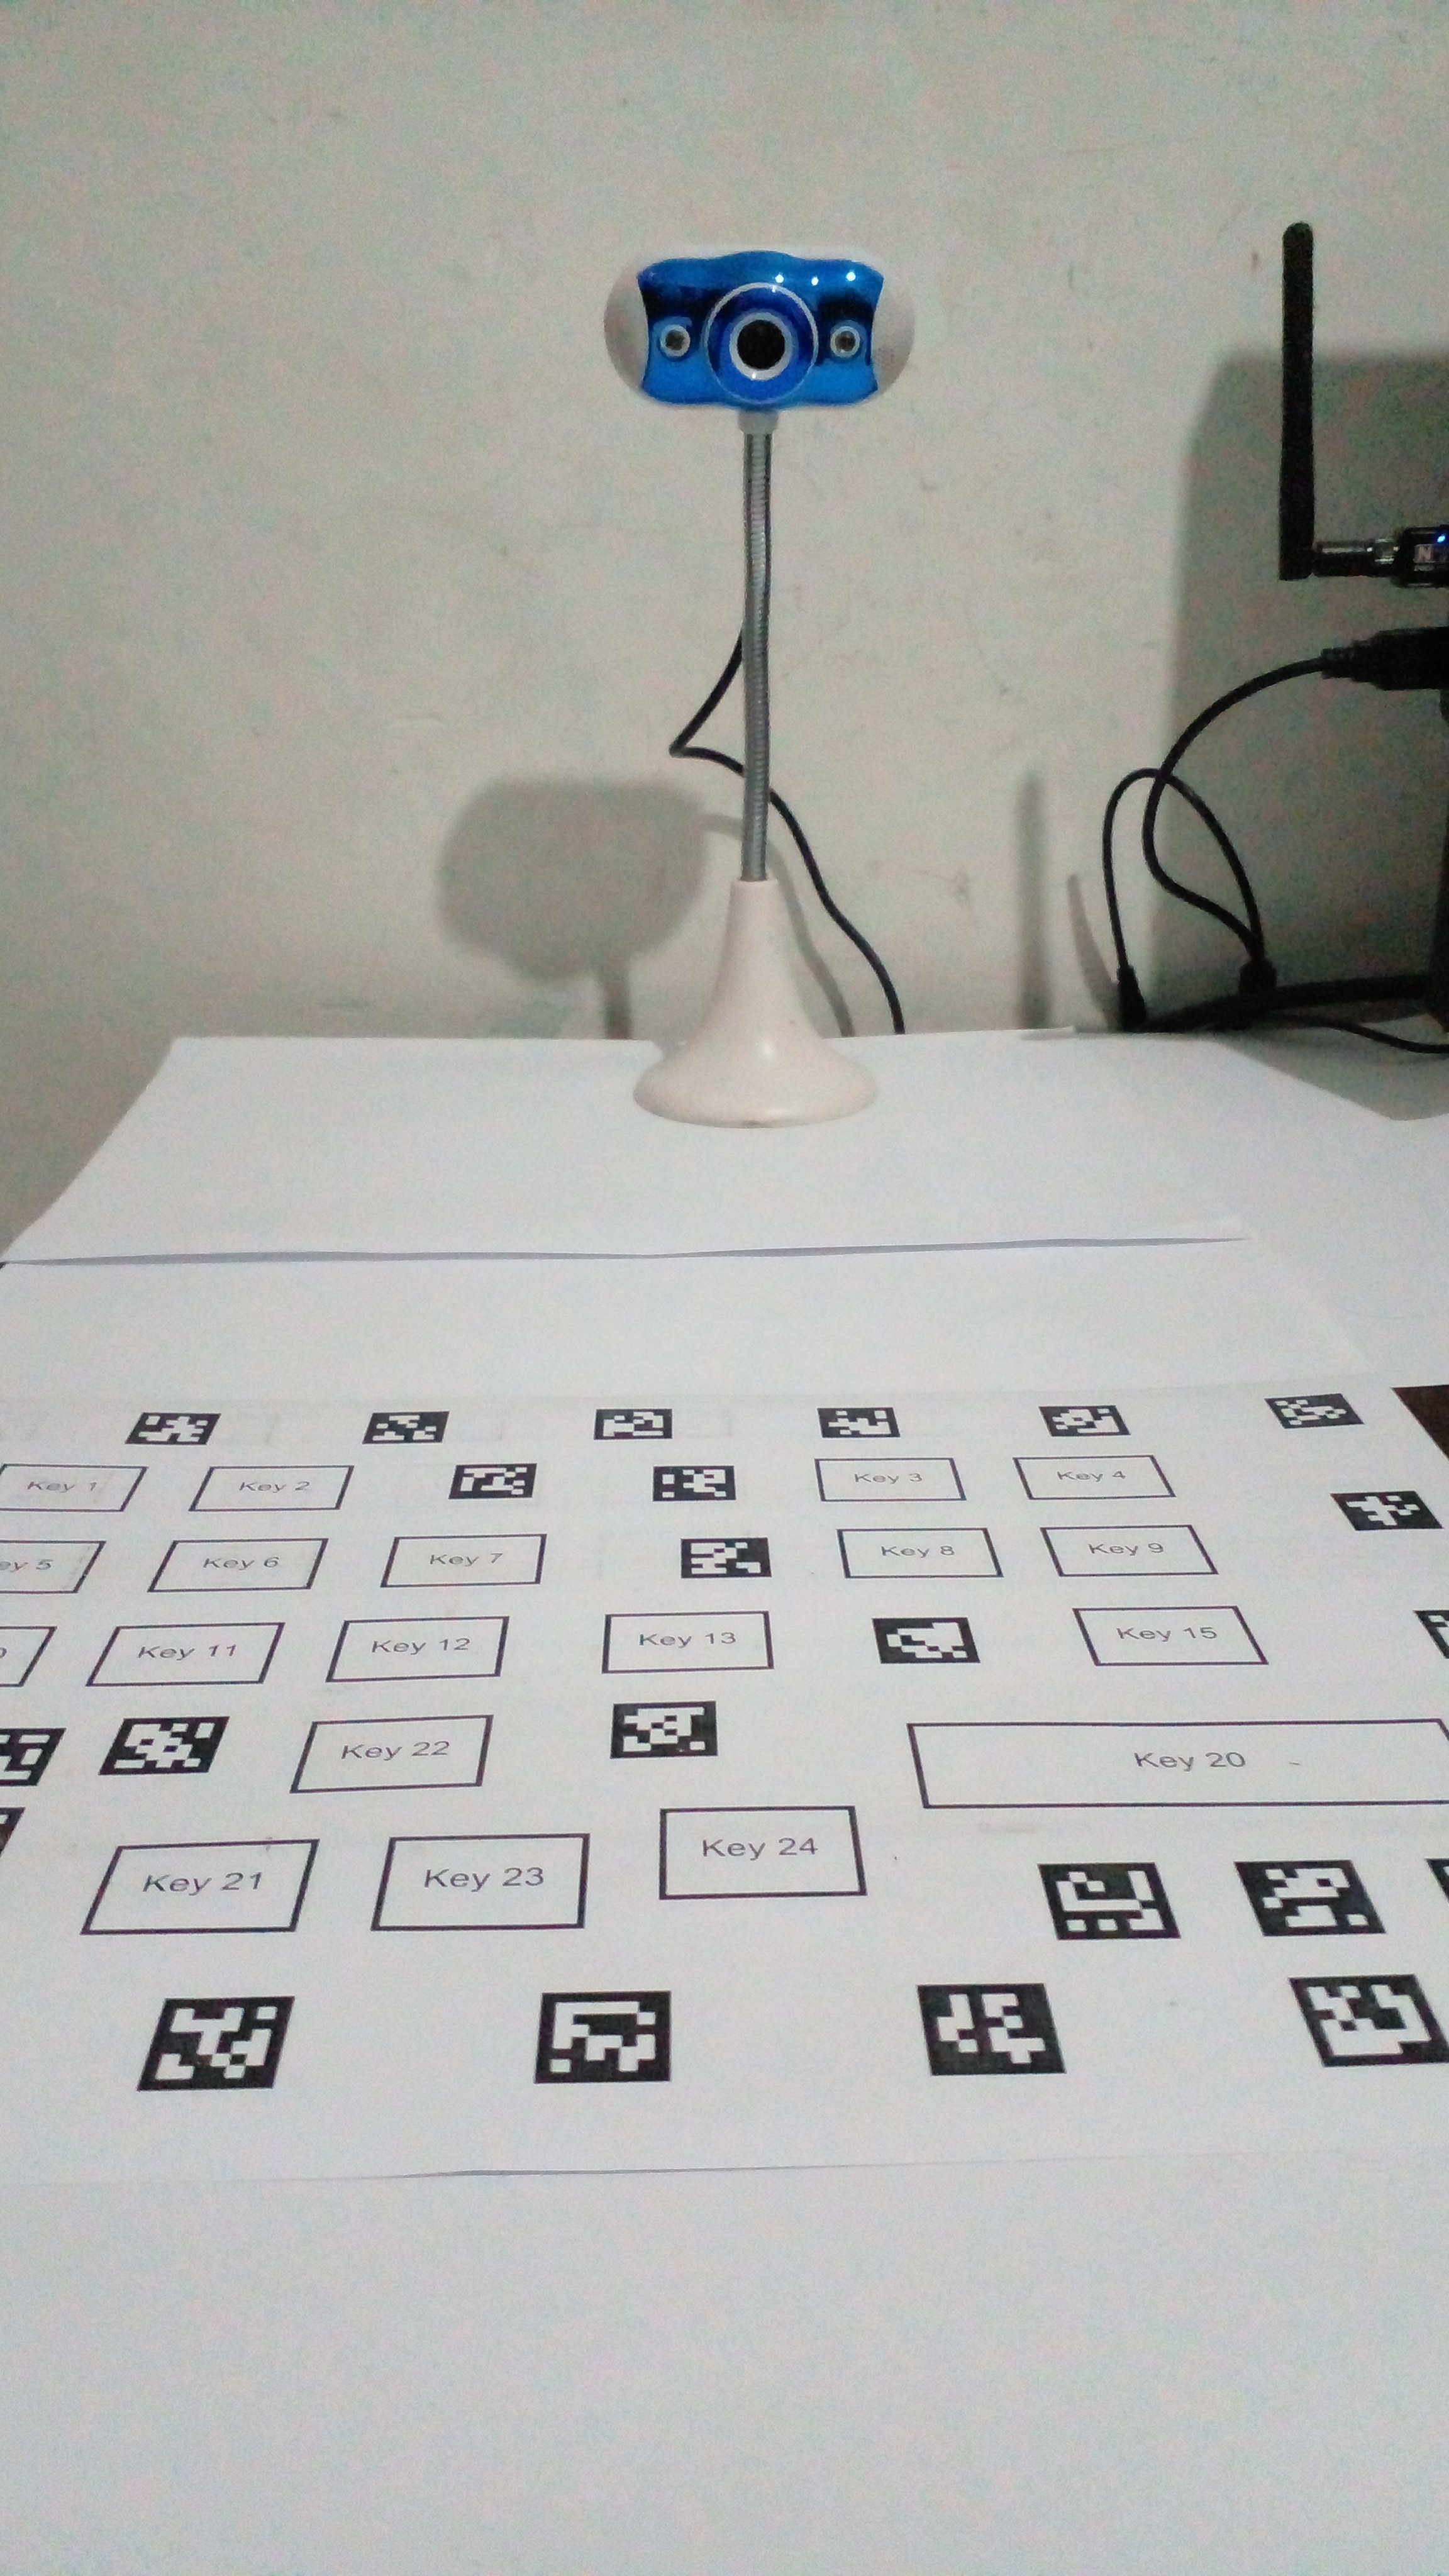
\includegraphics[width=0.72\textwidth]{figures/physical_setup_image_upright.jpg}
\caption{Physical experimental desk setup with monocular USB webcam mounted on an adjustable arm above the printed paper macro keyboard layout.}
\label{fig:appendix_physical_setup}
\end{figure}

\newpage

\section{Printable Vector Layout Artifact}
\label{sec:appendix_printable_layout}
Figure~\ref{fig:appendix_printable_pdf} shows the printable PDF layout created by Application~1 (Layout Designer). The layout is saved at 300~DPI so it prints clearly on normal A4 paper using any normal office printer. Four AprilTag markers (IDs 0, 1, 2, and 3) are placed at the corners. The middle area contains the custom macro keys with clear border lines and button names.

\begin{figure}[htbp]
\centering
\includegraphics[width=0.88\textwidth]{figures/printable_layotu_pdf_image.png}
\caption{Exported 300~DPI vector PDF layout embedded with AprilTag border fiducials ready for standard desktop paper printing.}
\label{fig:appendix_printable_pdf}
\end{figure}
